\documentclass{article}
\usepackage{amsmath}
\usepackage{enumerate}
\usepackage{multicol}
\usepackage{listings}
\usepackage{graphicx}
\usepackage[margin=1in]{geometry}
\begin{document}
\begin{center}
\textbf{\textit{CPSC 330 Midterm Review}}\\
\end{center}

\section*{Hardware and Performance}
\hrule
\noindent\\
\indent The following equations are given:
\begin{enumerate}
\item $CPU\ Time = \frac{Clock\ Cycles}{Clock\ Rate}$
\item $CPU\ Time = Instructions \times \frac{Cycles}{Instruction} \times \frac{Seconds}{Cycle}$
\item $CPU\ Time = Clock\ Cycles \times Cycle\ Time$
\item $CPI = \frac{Clock\ Cycles}{Instructions}$
\item $CPU\ Time = Instruction\ Count \times CPI \times Cycle\ Time$
\item $CPU\ Time = Instruction\ Count \times \frac{CPI}{Clock\ Rate}$
\item $(Clock\ Cycles)_{Total} = \sum_{i = 1}^{n}\left(CPI_{i} \times Count_{i}\right)$
\item $MIPS = \frac{Instruction\ Count}{CPU\ Time \times 10^{6}}$
\item $Power = Capacitive\ Load \times (Voltage)^{2} \times Frequency$
\end{enumerate}


\hrule
\noindent \\
\indent \textit{\textbf{Question 1:}} How can we improve performance?\\
\noindent \textit{\textbf{Solution:}} There are several factors that can help to improve performance of a system. Consider the following equation:
\[
\frac{seconds}{program} = \frac{cycles}{program} \times \frac{seconds}{cycle} = \frac{cycles/program}{clock\ rate}
\]
\noindent From this equation, we can tell that there are a few ways to increase performance. For example, we can
\begin{enumerate}
\item We can \textbf{decrease} the number of cycles in a program. If we look at the right-most side of the equation, we can see that decreasing the numerator will decrease the $\frac{seconds}{program}$.
\item By a similar argument, we can say that \textbf{increasing} the clock rate will also decrease the $\frac{seconds}{program}$.
\item Increasing the cycles is the same as \textbf{decreasing} the clock cycle time.
\end{enumerate}


\hrule
\noindent \\
\indent \textit{\textbf{Question 2:}} Suppose we have two implementations of the same ISA on machines $A$ and $B$. Machine $A$ has a clock rate of 4GHz and a CPI of 2.0, and machine $B$ has a clock rate of 2GHz and a CPI of 1.2. If we run the same program on both machines, which machine is faster, and by how much?\\
\noindent \textit{\textbf{Solution:}} Recall the equations we have above. In our case, we will be looking at equation [5]. Since the program is the same on both machines, the number of instructions will cancel out. We want to find the ratio of the speeds, and then convert them into percentages.
\begin{align*}
\frac{CPU\ Time_{A}}{CPU\ Time_{B}} &= \frac{
Instruction\ Count \times \frac{CPI_{A}}{Clock\ Rate_{A}}
}{
Instruction\ Count \times \frac{CPI_{B}}{Clock\ Rate_{B}}
}\\
&= \frac{
\frac{CPI_{A}}{Clock\ Rate_{A}}
}{
\frac{CPI_{B}}{Clock\ Rate_{B}}
}\\
&= \frac{CPI_{A}\times Clock\ Rate_{B}}{Clock\ Rate_{A}\times CPI_{B}}\\
&= \frac{2.0 \times 2}{1.2 \times 4}\\
&= 83.3\%
\end{align*}
\noindent So, Machine A is $83.3\%$ faster than machine B.\\
\hrule
\newpage


\indent \textit{\textbf{Question 3:}} Two computers, $C_{1}$ and $C_{2}$ have the following metrics when running the same program:
\begin{center}
\begin{tabular}{|c|c|c|}
\hline
& Computer $C_{1}$ & Computer $C_{2}$\\ \hline
\# Instructions & 10 billion & 8 billion\\ \hline
Clock Rate & 4GHz & 4GHz\\ \hline
CPI & 1.0 & 1.1\\ \hline
\end{tabular}
\end{center}
\noindent Which computer is faster, and which has higher MIPS?\\\\
\textit{\textbf{Solution:}} Let's address the first part of the question: \textit{Which computer is faster?}. To do this, we can use equation [6]. We will have the following:
\begin{alignat*}{3}
CPU\ Time_{1} &= 10e9 \times \frac{1.0}{4e9} \qquad\qquad CPU\ Time_{2} &&= 8e9 \times \frac{1.1}{4e9}\\
&= \frac{10}{4} &&= \frac{8.8}{4}\\
&= 2.5 &&= 2.2
\end{alignat*}
\noindent So we can see that $C_{2}$ is faster than $C_{2}$. Now lets answer the second part of the conversation. To find the MIPS, we need to use [8]:
\begin{alignat*}{3}
MIPS_{1} &= \frac{10e9}{4e9} \qquad\qquad MIPS_{2} &&= \frac{8e9}{4e9}\\
&= 2.5 &&= 2
\end{alignat*}
\noindent And we are done.\\


\hrule
\noindent \\
\indent \textit{\textbf{Question 4:}} A compiler designer is trying to decide between two code sequences for a particular machine. Based on the hardware implementation, there are three different classes of instructions: Class A, Class B, and Class C, and they require one, two, and three cycles, respectively.\\
\indent \indent The first code sequence has 5 instructions: 2 of A, 1 of B, and 2 of C\\
\indent \indent The second sequence has 6 instructions: 4 of A, 1 of B, and 1 of C\\
\noindent Which sequence will be faster, and by how much? What is the CPI for each sequence?\\\\
\textit{\textbf{Solution:}} Recall equation [4]. It tells us that the CPI will be equal to the clock cycles divided by the number of instructions. To solve this problem, we need to realize that the total number of cycles will be the sum of each cycle. In other words, we have
\begin{alignat*}{3}
CPI_{1} &= \frac{1 + 1 + 2 + 3 + 3}{5} \qquad\qquad CPI_{2} &&= \frac{1 + 1 + 1 + 1 + 2 + 3}{6}\\
&= \frac{10}{5} &&= \frac{9}{6}\\
&= 2 &&= 1.5
\end{alignat*}
\noindent So we have the CPI for each sequence. Since we have the same machine, the ratios for both [6] and [5] will have elements that cancel out. Let's use [5] in this case, as it will be simpler.
\begin{align*}
\frac{CPU\ Time_{1}}{CPU\ Time_{2}} &= \frac{5 \times 2 \times Cycle\ Time}{6 \times 1.5 \times Cycle\ Time}\\
&= \frac{10}{9}\\
&= 1.11
\end{align*}
\noindent This tells us that sequence 1 is faster than sequence 2, and in fact it is 11\% faster.\\
\hrule
\newpage


\indent At this point, we will introduce a table that shows us what factors affect the CPU Time. Recall from [5] that The number of instructions, the CPI, and the cycle time all influence the CPU Time. An ``X`` implies that the CPU time factor is directly affected, and a $\sim$ implies that it indirectly affects a factor of the CPU Time.
\begin{center}
\begin{tabular}{|c|c|c|c|}
\hline
& \# Instructions & CPI & Clock Cycles \\ \hline
Algorithms & X & $\sim$ & \\ \hline
Language & X & $\sim$ & \\ \hline
Compiler & X & X & \\ \hline
ISA & X & X & X \\ \hline
Technology & & & X\\ \hline
\end{tabular}
\end{center}
\hrule
\noindent \\
\indent \textit{\textbf{Question 5:}} Consider the following table which describes the attributes of a certain machine:
\begin{center}
\begin{tabular}{|c|c|c|c|}
\hline
Op & Frequency & CPI & Frequency $\times$ CPI\\ \hline
ALU & 50\% & 1 & 0.5\\ \hline
Load & 20\% & 5 & 1.0\\ \hline
Store & 10\% & 3 & 0.3\\ \hline
Branch & 20\% & 2 & 0.4\\ \hline
& & & $\sum = 2.2$\\ \hline 
\end{tabular}
\end{center}
\begin{enumerate}[\qquad\qquad a.]
\item How much faster would the machine be if a better data cache reduced the average load time to 2 cycles?
\item How does this compare with using branch prediction to shave a cycle off the branch time?
\item What if two ALU instructions could be executed at once?
\end{enumerate}
\noindent \textit{\textbf{Solution:}} Let's start with part \textit{a}. To solve this, we will have to recalculate the total sum of Frequency $\times$ CPI. Luckily, all the values will stay the same except of the CPI for the load, which is being changed to 2. The new value for Frequency $\times$ CPI is now $0.2 \times 2$, or 0.4. This makes the total sum 1.6, and the ratio of the old sum to the new sum is $2.2 : 1.6$, or 37.5\%.\\\\
\noindent We will do the same thing for part \textit{b}. In this case we will have one less cycle for the branch time, bringing the Frequency $\times$ CPI for the Branch operation to 0.2. Our new sum is 2.0, which means that we have a ratio of $2.2 : 2.0$, or 10\%\\\\
\noindent Part \textit{c} is a little different, but not too far off from \textit{a} and \textit{b}. In this case, it's not the CPI that's changing, but rather the frequency. We can process 2 ALU instructions at once, so the frequency will be half of what it currently is. In other words, we will have a frequency of 25\%, instead of 50\%. This makes the Frequency $\times$ CPI for the ALU 0.25, and the total sum is now 1.95. Now we have a ratio of $2.2 : 1.95$, or 12.8\%.\\
\hrule
\newpage


\section*{MIPS Assembly}
\hrule
\noindent\\
\indent \textit{\textbf{Question 1:}} Translate the following piece of pseudocode into MIPS instructions, with \$t0 and \$t1 as temporary registers.
\begin{center} 
\begin{tabular}{c}
\begin{lstlisting}
f = (g + h) - (i + j);
\end{lstlisting}
\end{tabular}
\end{center}
\noindent \textit{\textbf{Solution:}} This is simple. Just remember that R-Type MIPS instructions (e.g. add, sub, ...)  take three arguments: the register to store the value into, the left-hand operand, and the right-hand operand. We have as follows:
\begin{center} 
\begin{tabular}{c}
\begin{lstlisting}
add $t0, g, h
add $t1, i, j
sub f, $t0, $t1
\end{lstlisting}
\end{tabular}
\end{center}
\hrule
\noindent \\


\indent \textit{\textbf{Question 2:}} Assume A is an array of 100 words. Variables g and h are associated with registers \$s1 and \$s2 and the starting (base) address of the array is in \$s3. Use \$t0 as a temporary register. Translate the following pseudocode into MIPS assembly.
\begin{center} 
\begin{tabular}{c}
\begin{lstlisting}
g = h + A[8];
\end{lstlisting}
\end{tabular}
\end{center}
\noindent \textit{\textbf{Solution:}} The trick here is to remember that in a 32-bit system, each address in memory is separated by 4 bytes. In other words, if you want to access the 9th index of A, you need to move four spaces in memory, rather than just one. We also need to remember the syntax for an offset. We have two ways of doing this: we can use the add instruction on the address, or we can specify an offset. Since the base address of the array is stored in \$s3, we need to offset by $8 \times 4$, or 32. We will have the following:
\begin{center} 
\begin{tabular}{c}
\begin{lstlisting}
lw $t0, 32($s3)
add $s1, $s2, $t0
\end{lstlisting}
\end{tabular}
\end{center}
\hrule
\noindent \\


\indent Before we continue, lets talk about MIPS instructions in more detail. MIPS is built for a 32-bit system, and as a result, MIPS instructions are all 32 bits. We have three types of instructions, R-Type, I-Type, and J-Type. R-Type instructions deal with arithmetic operations, such as add, sub, mult, slt, and the like. I-Type instructions deal with memory, and include instructions like lw, sw, la, and others. I-Type also deals with instructions that load values immediate J-Type instructions deal with branching and jumps, which includes instructions such as j, beq, and bne. All MIPS instructions have the same number of bits, which is best illustrated by the R-Type format:
\begin{center}
\begin{tabular}{|c|c|c|c|c|c|}
\hline
op - 6 bits & rs - 5 bits & rt - 5 bits & rd - 5 bits & shamt - 5 bits & funct - 6 bits \\ \hline
\end{tabular}
\end{center}
\noindent Note that the instruction type changes the meaning of the bits. For example, consider an I-Type instruction as follows:
\begin{center} 
\begin{tabular}{c}
\begin{lstlisting}
lw $t0, 400($t1)
\end{lstlisting}
\end{tabular}
\end{center}
\noindent The opcode for this instruction is $(35)_{10}$ (you would have to look this up in a table). The values for rs and rt are $9_{10}$ and $8_{10}$, respectively. However, we won't use the last 16 bits the same way we would use it for an R-Type instruction. For an I-Type instruction, the last 16 bits are used for the offset. In this case, they 32 bit representation of this instruction would look like:
\begin{center}
\begin{tabular}{|c|c|c|c|c|c|}
\hline
$(35)_{10}$ - 6 bits & $(9)_{10}$ - 5 bits & $(8)_{10}$ - 5 bits & \multicolumn{3}{|c|}{$(400)_{10}$  - 16 bits} \\ \hline
\end{tabular}
\end{center}
\noindent Now consider the R-Type add instruction:
\begin{center} 
\begin{tabular}{c}
\begin{lstlisting}
add $t0, $s2, $t0
\end{lstlisting}
\end{tabular}
\end{center}
\noindent Which would result in the following bits: 
\begin{center}
\begin{tabular}{|c|c|c|c|c|c|}
\hline
$(0)_{10}$ - 6 bits & $(18)_{10}$ - 5 bits & $(8)_{10}$ - 5 bits & $(8)_{10}$ - 5 bits & $(0)_{10}$ - 5 bits & $(32)_{10}$ - 6 bits \\ \hline
\end{tabular}
\end{center}
\noindent As you can see, an R-Type instruction uses each section, while the I-Type does not. Let's look at a J-Type instruction, which will only have two sections
\begin{center} 
\begin{tabular}{c}
\begin{lstlisting}
j branchname
\end{lstlisting}
\end{tabular}
\end{center}
\noindent This instruction results in the following table:
\begin{center}
\begin{tabular}{|c|c|c|c|c|c|}
\hline
$(2)_{10}$ - 6 bits &  \multicolumn{5}{|c|}{$(24)_{10}$ - 26 bits}\\ \hline
\end{tabular}
\end{center}
\noindent It's worth mentioning that there are also FR-Type and FI-Type instructions. The difference between FR/FI-Type and R/I-Type is that FR/FI-Type deal with floating point numbers. The instruction format is the same, but rather than rs, rt, rd, and shamt, we have fmt, ft, fs, and fd. \\
\hrule
\noindent \\


\indent \textit{\textbf{Question 3:}} Given the following MIPS code, create a trace table:
\begin{center} 
\begin{tabular}{c}
\begin{lstlisting}
0x400:a addi 	$t0, $zero, 3
0x404:b add 	$v0, $t0, $t0 
0x408:c addi 	$t0, $t0, -1
0x40c:d bne 	$t0, $zero, b
0x410:e j 	e
\end{lstlisting}
\end{tabular}
\end{center}
\noindent \textit{\textbf{Solution:}} For each instruction, we will analyze the values of the program counter and the \$t0 and \$v0 registers. Let's take it instruction by instruction:
\begin{enumerate}[a)]
\item 
\begin{lstlisting}
0x400:a addi $t0, $zero, 3
\end{lstlisting}
\noindent In this case, there is nothing in \$v0, so we just forget about it for now. The program counter is the element that holds the current address in memory, so in this step it contains 0x400. Finally, we are adding $3 + 0$ and storing the value in \$t0, which makes \$t0 = 3.
\item
\begin{lstlisting}
0x404:b add $v0, $t0, $t0 
\end{lstlisting}
\noindent Now, we are adding \$t0 to itself and storing the value in \$v0. We know from \textit{a)} that \$t0 contains 3, so \$v0 = 6. The program counter has increased by 4.
\item 
\begin{lstlisting}
0x408:c addi $t0, $t0, -1
\end{lstlisting}
\noindent We are essentially decrementing \$t0 here, so \$t0 will contain 2. \$v0 is unchanged, and the program counter is incremented by 4.
\item 
\begin{lstlisting}
0x40c:d bne $t0, $zero, b
\end{lstlisting}
\noindent Here is where things get interesting. Recall that a ben instruction says that if (in this case) \$t0 is not equal to \$zero, then goto b. Since \$t0 is not 0, we jump back up to b. The program counter in this step is incremented by 4, and \$v0 and \$t0 do not change.
\end{enumerate}
\noindent Now we can continue to fill out the table. We know that it will continue to branch until \$t0 holds the value of \$zero. The table is as follows:
\begin{center}
\begin{tabular}{|c|c|c|c|c|c|c|c|c|c|c|c|}
\hline
\multicolumn{12}{| l |}{Trace Table}\\ \hline
Step & 1 & 2 & 3 & 4 & 5 & 6 & 7 & 8 & 9 & 10 & 11\\ \hline
pc & 0x400 & 0x404 & 0x408 & 0x40c & 0x404 & 0x408 & 0x40c & 0x404 & 0x408 & 0x40c & 0x410 \\ \hline
\$t0 & 3 & 3 & 2 & 2 & 2 & 1 & 1 & 1 & 0 & 0 & 0\\ \hline
\$v0 & - & 6 & 6 & 6 & 4 & 4 & 4 & 2 & 2 & 2 & 2\\ \hline
\end{tabular}
\end{center}
\hrule
\newpage


\section*{The ALU in Hardware}
\hrule
\noindent\\
\indent Now we will talk about the ALU in terms of hardware. For the next few problems, we will consider the following diagram, which is one ALU unit. In a 32-bit system, there would be (you guessed it) 32 of these units.\\
\begin{center}
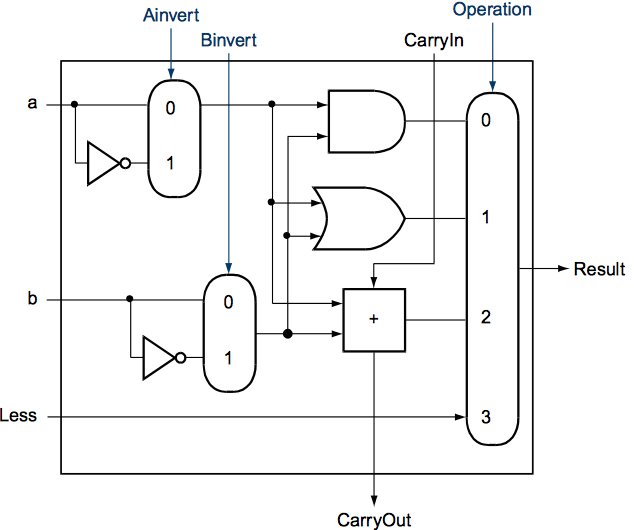
\includegraphics[scale=0.35]{alu2}
\end{center}
\noindent We actually can observe quite a lot about the ALU pictured above. For example, lets imagine that we have $a = 1$, and $A\ invert = 1$. Then we know that the value from the \textit{MUX} that handles the $a$ input will output 0, since the select line choses the inverted $a$. The same can be said for the \textit{MUX} that handles the $b$ signal. There is also another \textit{MUX} that handles the resulting output of the ALU.\\
\indent You can imagine that in a 32-bit system, this arrangement would not be very efficient. We won't go into too much detail, but the strategy to implement the ALU in a 32-bit (or even 64-bit) is \textbf{not} to align each of the ALU's in series. Rather, the hardware uses a \textit{carry lookahead} to help make the system more efficient Let's talk about how different instructions are implemented in the ALU.\\
\hrule
\noindent \\


\indent \textit{\textbf{Question 1:}} Describe how the following instruction could be implemented in the ALU:
\begin{center}
\begin{tabular}{c}
\begin{lstlisting}
slt $t0, $t1, $t2
\end{lstlisting}
\end{tabular}
\end{center}
\noindent \textit{\textbf{Solution:}} Recall what the $slt$ instruction does. If \$t1 $<$ \$t2, then \$t0 receives the value of 1; otherwise, \$t0 gets 0. So the question we are really asking is ``How can the ALU determine if a value is less than another value?'' We can tell when two values are equal by subtracting them and seeing if the value is zero, so that takes care of the case where the values are equal. Now we need a way to determine if \$t1 $>$ \$t2. To do this, we can subtract \$t2 from \$t1, and if the value is greater than $0$, then we know that \$t1 $>$ \$t2. If neither of these are true, then we set all the bits in \$t0 to 0. The hardware is implemented using adders. For the hardware to take the 2's compliment, it must invert the and then add 1 to the result. For example, we can try the following:
\begin{enumerate}[a)]
\item Let $a = 0011110$ and $b = 0101110$. Determine the value of $f$ given the following:
\begin{center}
\begin{tabular}{c}
\begin{lstlisting}
slt f, a, b
\end{lstlisting}
\end{tabular}
\end{center}
\end{enumerate}
\noindent Remember that in order to subtract binary numbers, we need to find the 2's compliment of the second number and add it into the first. Alternatively, we can convert the numbers into base 10 and then back into base 2. We will do it the second way here. Changing both into decimal give us:
\begin{alignat*}{3}
(0011110)_{2} &= (0 + 0 + 2^{4} + 2^{3} + 2^{2} + 2 + 0)_{10} \qquad\qquad (0101110)_{2} &&= (0 + 2^{5} + 0 + 2^{3} + 2^{2} + 2 + 0)_{10}\\
&= (30)_{10} &&= (46)_{10}
\end{alignat*}
\noindent It's very easy to see here that $a < b$, so we know that $f = 1$. Now let's try it with the 2's compliment, since the hardware cannot change binary into decimal. We only need to change $a$ into the 2's compliment.
\[a:\ 0011110 \to 1100001\]
\begin{center}
\begin{tabular}{c r}
& 1100001 \\
+ & 1 \\ \hline
& 1100010
\end{tabular}
\end{center}
\noindent Now we add $b$ to the 2's compliment of $a$:
\begin{center}
\begin{tabular}{c r}
& 1100010 \\
+ & 0101110 \\ \hline
& 10010000
\end{tabular}
\end{center}
\noindent Note that we have a signed int here, so we can just ignore the signed bit. This gives us what we expected: that is $a < b$, or that $b - a > 0$. Thus, f will be set to 00000001.\\
\hrule
\noindent\\ 


\indent \textit{\textbf{Question 2:}} Describe how the following instruction could be implemented in the ALU:
\begin{center}
\begin{tabular}{c}
\begin{lstlisting}
beq $t0, $t1, label 
\end{lstlisting}
\end{tabular}
\end{center}
\noindent \textit{\textbf{Solution:}} This is a very simple problem. We already looked at the $slt$ instruction, and we stated that we can tell if $\$t0 == \$t1$ if their difference is zero, and the program counter will change to the address of \textit{label}.
\end{document}